%# -*- coding: utf-8-unix -*-
%%==================================================
\chapter{Start here: 入口级网站和应用}
\label{necessary_resources}

\begin{flushright}
    ——据说99\%的博士生都收藏了这些
\end{flushright}    

\section{网站}
\begin{itemize}
    \item 西浦校内网站导航:\url{https://guide.xjtlu.edu.cn}
    \item 个人信息门户ebridge:\url{https://ebridge.xjtlu.edu.cn}
    \item 利物浦信息门户Liverpool Life:\url{https://liverpool-life.liverpool.ac.uk}
\end{itemize}

\section{公众号}

\begin{table}[H]
    \begin{tabular}{ccc}
        \begin{subfigure}{0.25\columnwidth}
            
\includegraphics[width=\linewidth]{author-folder/Kai.Wu/qrcode_XJTLU-China_1.jpg} \caption{学校公众号}
        \end{subfigure} \hfill
        \begin{subfigure}{0.25\columnwidth}
            
\includegraphics[width=\linewidth]{author-folder/Kai.Wu/qrcode_XJTLU_library_1.jpg} \caption{图书馆}
        \end{subfigure} \hfill
        \begin{subfigure}{0.25\columnwidth}
            
\includegraphics[width=\linewidth]{author-folder/Kai.Wu/qrcode_student_service.jpg} \caption{学生服务(一站式)}
        \end{subfigure} \hfill
        \begin{subfigure}{0.25\columnwidth}
            
\includegraphics[width=\linewidth]{author-folder/Kai.Wu/qrcode_IT.jpg} \caption{IT}
        \end{subfigure} \hfill
    \end{tabular}
\end{table}

另外,各学院可能有自己的公众号,由于太多无法一一列出,可自行在微信搜索,例如 “西浦\ {学院名}" 或者 "西交利物浦\ {学院名}"

\section{手机APP}
\url{https://guide.xjtlu.edu.cn/How-to-install-the-XJTLU-APP.html}

\section{常用资源位置位置}
\subsection{校园地图:某栋楼在哪里}
见本攻略最后一页。或者微信搜“西浦地图”小程序

\subsection{官方PGR Handbook电子版、学校政策、校规}
登录ebridge,在中间的PGR Policies, Procedures and Forms里

\subsection{校历:哪天放假}
\begin{figure}[H]
    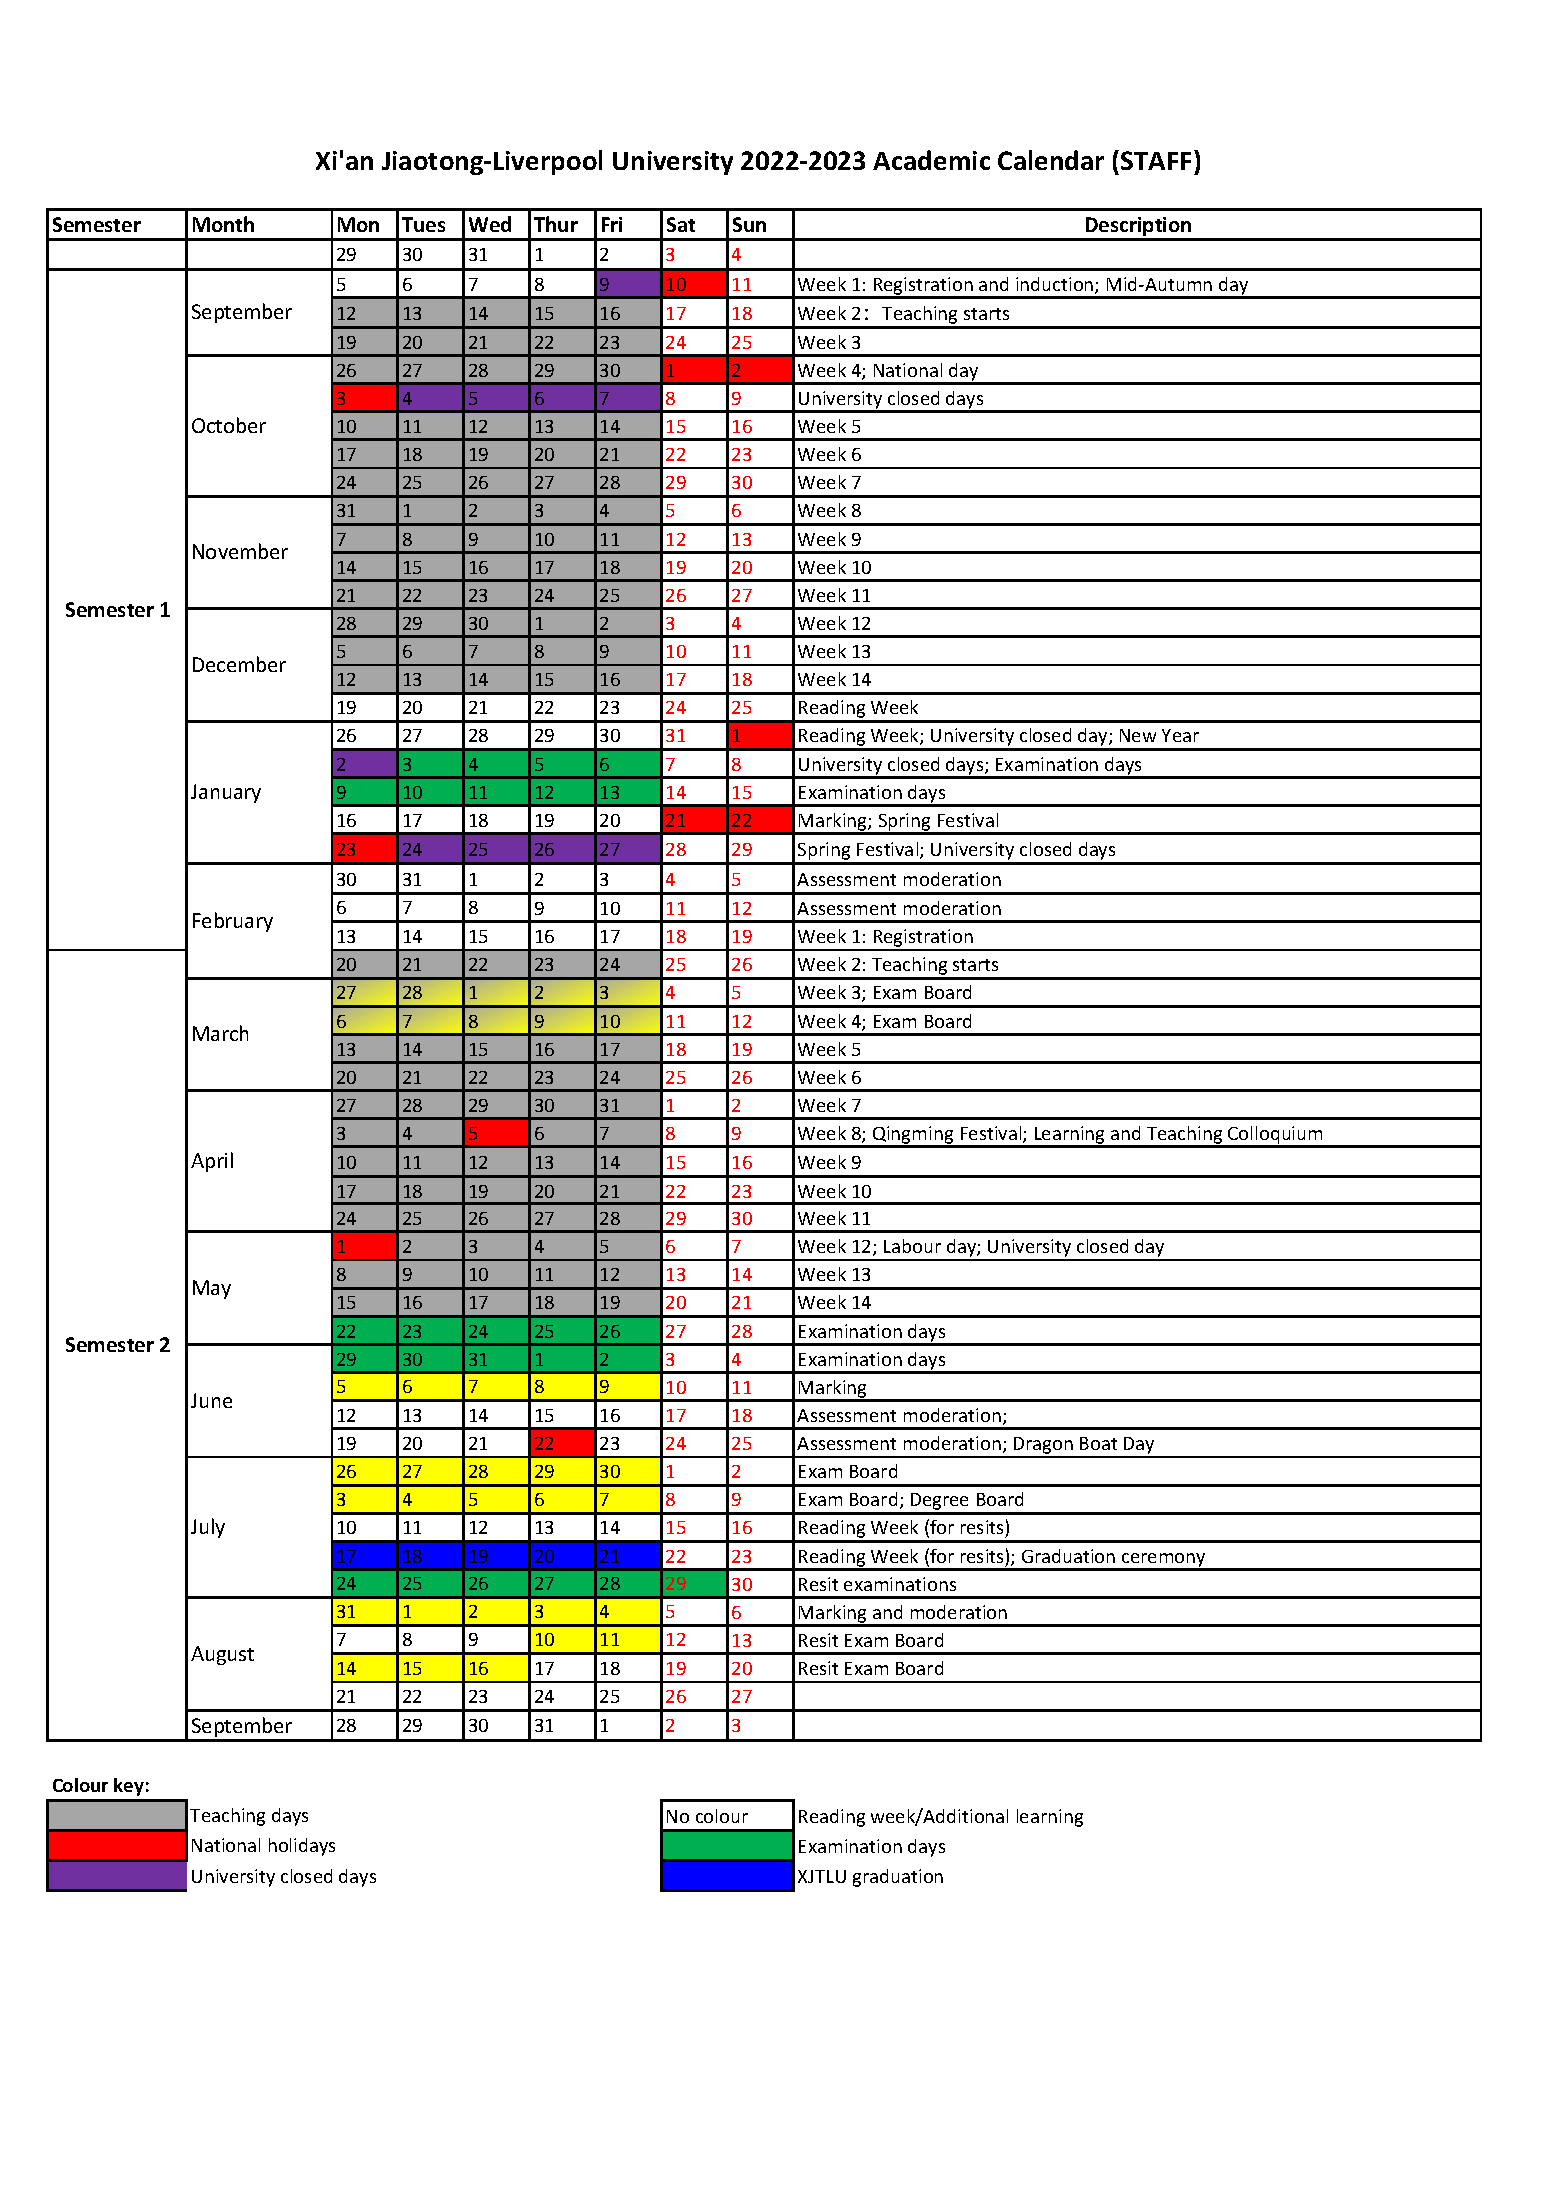
\includegraphics[width=\columnwidth]{author-folder/Kai.Wu/Academic_Calendar-202223.pdf}
\end{figure}


